\chapter{Development of RFID application for management and tracking assets and drugs}
\label{Kap3}

The third and last chapter of this Bachelor Thesis gives information about the development process of a RFID tracking application. In the following, the system's requirements \ref{requirements} are described. Additionally, all used platforms and technologies are mentioned in section \ref{platforms}. Then, the specific development process \ref{app_development} is depicted which demonstrates the software's architecture introducing some diagrams. Lastly, several planned tests as well as their test results are discussed in section \ref{tests}.

\section{Proposed solution of application}\label{requirements}

\subsection{Aim of developed application}

The aim of the proposed system is to improve logistics and the management of drugs in hospitals. Considering the risk of errors or mistakes that might occur when administering drugs to patients, the developed mobile application can prevent these situations. Furthermore, when patients are in a critical situation, the system offers the possibility to respond faster to emergencies as well as to improve patients' monitoring. Finally, the placement and usage of medical assets can be pursued and controlled better. 

The above mentioned reasons lead to the necessity of disposable, low cost RFID tags which might be tagged to patients, drugs and medical assets. Moreover, there has to be established a network between the mobile devices, the RFID reader and the synchronizing software. 

\subsection{Scope of developed application}

\begin{figure}
\centering
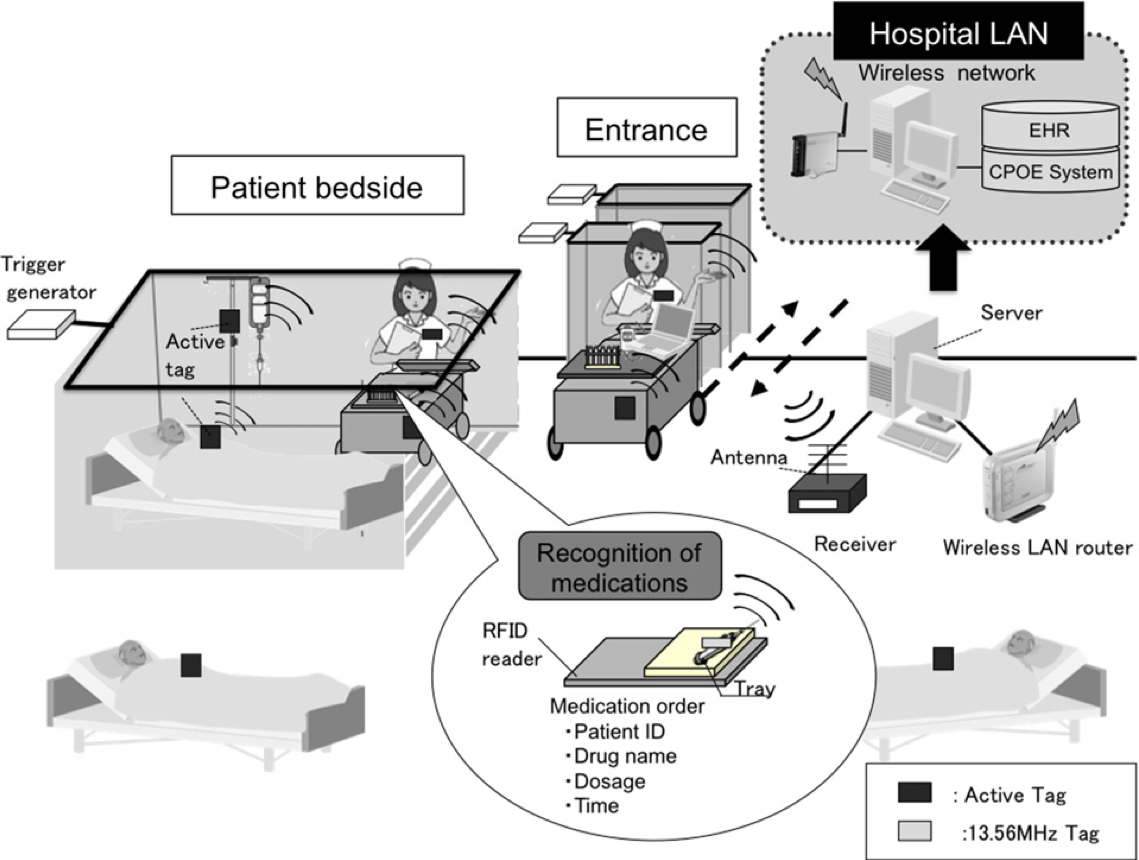
\includegraphics[width=\textwidth]{existing_apps} 
\caption{\label{fig:existing_apps} Existing RFID systems, based on 13.56 MHz short-range, inductive RFID tags} 
\end{figure}

In the past, RFID systems for management and logistics in hospitals were mostly based on 13.56 MHz short-range, inductive RFID tags.
Figure \ref{fig:existing_apps} gives an example of an existing RFID solution for management in hospitals. The given system has several advantages as well as disadvantages. On the one hand, as an advantage, using 13.56 MHz short-range, inductive RFID tags is a mature technology which is reliable. Further, the past solutions imply low-cost RFID tags which are easy to use. 
On the other hand, the disadvantages of the mentioned solutions are their complex infrastructure and the short-range. 

Therefore, this Bachelor Thesis proposes the use of 868 MHz frequency band while using a similar RFID architecture as the ones already tested and deployed. As an advantage of using 868 MHz frequency band, the proposed solution implies a longer range, wider coverage and the required hardware can be simplified. Further, the proposed solution of this Bachelor Thesis provides a mobile application for users which can be run on tablets and smartphones. 

\subsection{First system architecture} \label{firstconcept}

Figure \ref{fig:first_draft} describes the very first draft of the workflow of the application. Actually, it is not very precise but should help to describe the general scope of the medication tracking system. 
At the top of the picture, there is an Excel program which stores all data of the database and converts them into *.csv files. These converted files should be imported into the running MongoDB instance on the PC. 

On the same computer is running Matlab which is connected with the RFID reader. All along, MongoDB and Matlab are synchronizing each other. Beneath the PC, the figure shows the RFID reader which is connected to four antennas. At the bottom of figure \ref{fig:first_draft}, there are drawn four zoned antennas. Each zone can be seen as a different area or room and can represent a different state, e.g. 'entering' or 'leaving' the stockroom. In the bottom left corner, RFID tags detected sequentially by the antennas are shown. Each time, an antenna recognizes a tag, it sends the transmitted information to the reader which transfers the data to Matlab.  

\begin{figure}
\centering
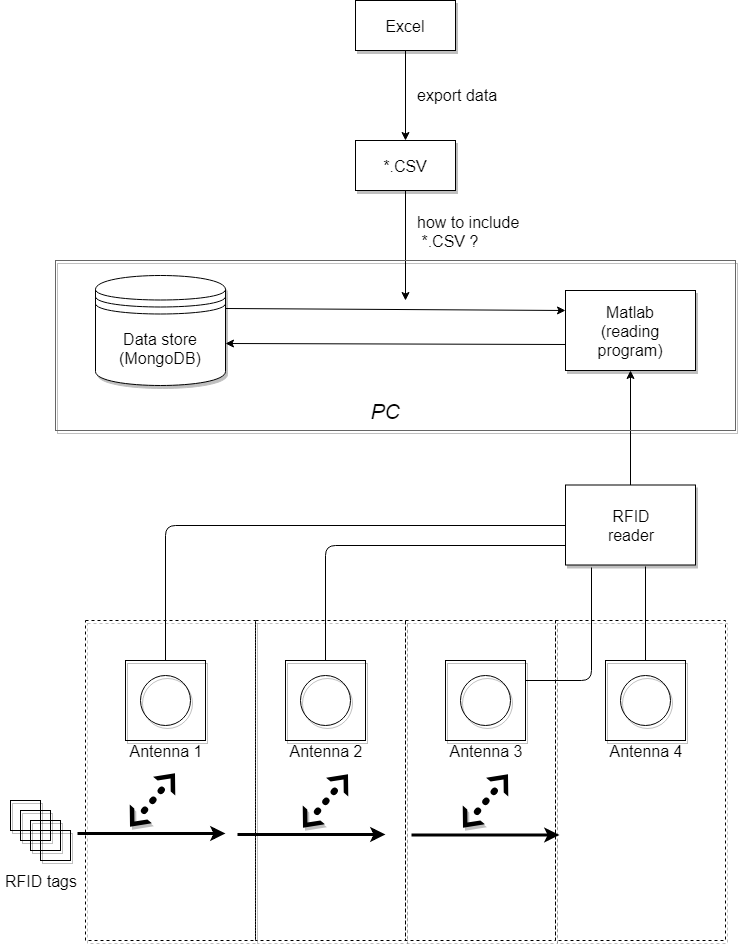
\includegraphics[width=\textwidth]{first_draft} 
\caption{\label{fig:first_draft}The first draft of the developed system} 
\end{figure}

This first concept was changed due to the use of the 'MongoDB' plugin, which offers Matlab \cite{matlab_mongodb}. This is much easier than exporting all received data from Matlab in *.csv format and then including it into MongoDB as *.csv data. Furthermore, it supports developing a very fast and real-time application which enables a higher data integrity because of the direct connection to the database.  

%talking about platforms in general, to get a common understanding 
\section{Used platforms and technologies} \label{platforms}

This section focuses on explaining the used technologies and frameworks for developping the mobile RFID application. Next, the framework 'NativeScript' which can be used for native mobile development will be explained. After that, section \ref{mongodb} discusses MongoDB, a document store. Finally, the Speedway Revolution RFID reader is presented. In the last section \ref{app_development} of this chapter the challenges as well as the user scenarios are shown. 

\subsection{Native Development with NativeScript} 

There are several ways to create a mobile application, like for example with Android Studio or iOS. But the challenge is to develop a hybrid solution for both systems at the same time.
To face that challenge, Nativescript has been established as an open-source project from Telerik in the last years \cite{nativescript}. 

The free and open source technology enables developers to easily build cross-platform native apps with either Javascript, Nativescript or by using Angular \cite{nativescript}. 
Regarding its design philosophy, Nativescript was designed to be approachable to developers from various backgrounds \cite{nativescript}. Moreover, it was designed to be both performant and giving access to native APIs, such as Android or iOS.

Figure \ref{fig:nsarchitecture} gives an impression of the general architecture of Nativescript applications. When developing such applications, one of the given frameworks can be used (e.g. '\{N\} Core', Angular or Vue). Additionally, several Nativescript plugins can be selected. Below the 'NativeScript Core Modules', there are located the 'NativeScript Runtimes' which have direct access to the Native system. By running several commands on the NativeScript \ac{CLI}, the developed Nativescript application can be executed on any physically connected device as well as on the installed emulator or in the cloud. 

\begin{figure}
\centering
\includegraphics[width=\textwidth]{ns-architecture} 
\caption{\label{fig:nsarchitecture}The architecture of NativeScript Applications, adopted from \cite{nsarchitecture}} 
\end{figure}

NativeScript applications can also be developed, built and run on the 'NativeScript Playground' \cite{nsplayground} which enables independent development. Moreover, NativeScript Playground is easier to handle because the application is executed in the Cloud. Generally, by offering a user-friendly surface, NativeScript Playground is appropriate for beginners who start developing native mobile applications.

\subsubsection{NativeScript Application Logic}

\begin{figure}
\centering
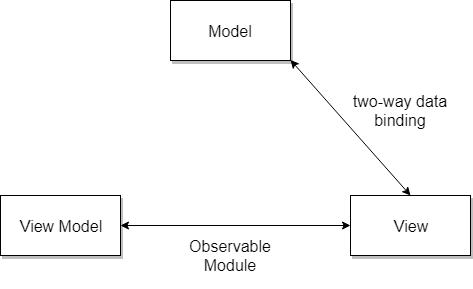
\includegraphics[width=\textwidth]{mvvm_ns} 
\caption{\label{fig:mvvm}The MVVM application logic, adopted from \cite{nativescript}} 
\end{figure}

NativeScript has a \ac{MVVM} application logic (see figure \ref{fig:mvvm}). In contrast to the popular \ac{MVC} application model, NativeScript offers two-way data binding by using the 'Viewmodel' \cite{nativescript}. In every NativeScript application, the model defines and represents data. After that, the data are bound to the view which represents them in a XML file. The 'ViewModel' contains the application logic and exposes all data to the view. 

The data between model and view can either be synchronized as one-way (default setting, the target property updates when a change in the source property occurs) or two-way data binding (all changes in the directions target-source and source-target will be transmitted). To enable the two-way data binding (see figure \ref{fig:mvvm}), the NativeScript Observable Module has to be implemented. 

According to the NativeScript Documentation \cite{nativescript}, the model files are called 'Code Behind' because they have the same name as the view file and are written in Javascript or Typescript. By adding attributes to any XML element in the view file, methods can be implemented in the related model file (in Javascript or TypeScript). 

\subsubsection{NativeScript Sidekick}\label{Native}

NativeScript Sidekick is a solution to run the developed application on unsupported platforms in the cloud. It uses both the local build infrastructure and the cloud build service. NativeScript Sidekick offers users to develop with the provided starter templates, to use verified plugins and to build the app in the cloud. Furthermore, NativeScript Sidekick enables developers to debug, test and refactor their application. 
To search for plugins and to manage these, developers can use the Nativescript Marketplace \cite{nsmarket}.

\subsection{NoSQL Technology: MongoDB}\label{mongodb}

NoSQL databases provide high availability, scalability and partitioning options \cite[p.25 ff.]{mongodb_edward}. Nevertheless, there are some disavantages when using MongoDB or any other document stores: For instance, both consistency and transactions are not supported. 

In contrast to relational databases, MongoDB does not consist of tables and rows, but of collections containing documents which make it both flexible and scalable \cite[p.25 ff.]{mongodb_edward}. Collections can be compared to tables in SQL, but are schemaless. Instead of having one unique schema within the same collection, every document can have its own set of fields, and common fields can store different values across documents.  

All data is stored in \ac{BSON} documents which assures that related data is placed all together in one place. BSON documents are JSON documents in binary-encoded format. It is the extended form of the JSON data model and is fast, high traversible and lightweight \cite[p.31 ff.]{mongodb_edward}. Moreover, JSON/BSON documents contain schema-less models. Each document stores data as key-value pairs, where the value can be left blank. Thus, users of MongoDB have to ensure and check the consistency of their data when adding new data.

One characteristic of MongoDB is the {\_} ID (key) which can be compared to the label or name of a column in RDBMS. If not explicitely specified by the user, a unique value is automatically generated and assigned to it by MongoDB. Basically, the key value is immutable and can be of any data type except arrays \cite[p.31 ff.]{mongodb_edward}.

Queries in a MongoDB database use the keys ({\_} ID) in documents which makes it possible to query documents spread across multiple servers. 
MongoDB uses primary-secondary replication, where the primary replication accepts the write requests. To be more precisely, if the write performance needs to be improved, the mechanism of sharding can be used. 

Sharding means that data will be split across multiple machines which are enabled to update different parts of datasets \cite[p.25 ff.]{mongodb_edward}. Besides, this mechanism is automatic in MongoDB, so that as more machines are added, the data is distributed automatically.

\subsection{Speedway Revolution RFID reader}

Concerning the implementation of the system, a Speedway R420 RAIN RFID READER \cite{speedway} with four antenna ports (extendable to 32 antennas with an Impinj Antenna Hub \cite{speedway}) was used. According to the manufacturer's web page \cite{speedway}, the Speedway R420 RAIN RFID READER can be connected to Impinj Autopilot technology which automatically optimizes the reader's operation for its environment. A test software can be downloaded from the Impinj web page  \cite{speedway}.

\subsection{Matlab}

Matlab is an interpreted language, usually used without an compilation step \cite[lesson 1]{introduction_matlab}. Actually, Matlab code is converted into machine code by an interpreter as the program is executed. Together with Java, Matlab counts to the high-level languages which on the one hand enables a faster code development but on the other hand limits the speed of execution. Matlab provides a large number of functions for common complicated operations in scientific computing (including engineering and analysis) and technical calculation.

Matlab provides important terminology, like e.g. variables (which contain three fundamental types: characters, real numbers, complex numbers), arguments, commands, command line, scripts, functions as well as comment \cite[lesson 1]{introduction_matlab}. 
One of the most common features of Matlab is its 'Debugger' \cite[lesson 8]{introduction_matlab} which is very useful for detecting unobvious errors.

\section{Application development} \label{app_development}

\subsection{Progress of development}

The development process can be divided into four steps which will be described in the next section. 

To begin with, initial tasks were devoted to learn how to create a NativeScript application from scratch. This phase included getting familiarized with the common NativeScript templates, views and framework logic as well as the data binding and data handling.

As a second task, the challenge of how to connect the NativeScript application to the backend (MongoDB) was faced. As a first solution, the connection to the MongoDB server was implemented using HTTP request/response. But in reality, there might be at least two devices (used by a nurse or doctor) which have to be connected to the database. For that reason, a socket connection (using the Socket.IO library) was established. With this technology, it was possible to connect multiple clients to the server instance and to synchronize all data in real-time.

After that, the third task was the handling of Matlab, its connection to MongoDB and to the Impinj RFID reader. In order to connect to the RFID reader, the Impinj Octane SDK was used. Thus, it was possible to configure several parameters for each antenna of the reader. This enables a precise identification of each antenna as well as the precise location of each detected item or drug. To give an example, antenna 1 placed in the hallway, whereas antenna 2 could be installed on the patient's room. 
Concerning the connection between RFID reader and MongoDB, there is a MongoDB plugin for Matlab. This provides several methods to connect to a MongoDB server and to retrieve and change the data from a specific database. Concluding these two implemented functionalities, Matlab serves both as a detection and information medium.

The last large task refers to the challenge of establishing a stable connection between all components (RFID reader, MongoDB database, NativeScript application and mobile devices). Therefore, two networks had to be created. The first network (LAN) connects the development laptop (MacOS), where both the NativeScript application and MongoDB database are running, to the Windows PC, where Matlab is running. Due to the use of .NET libraries in Impinj Octane SDK, Matlab had to be installed on a Windows PC. Another solution would be to run Windows on a VM on the MacOS developer machine (MacBook Pro Spring 2015, operating system: macOS High Sierra 10.13.5, RAM: 8 GB, Internal Storage: 128 GB), but unfortunately the RAM as well as disk space restricted the functionality of the VM. The second network that was installed was a private WLAN which connected all mobile devices (smartphones and tablets) with the MacOS developer machine. This connection enables receiving and transfering all data from the MongoDB database into the mobile app. To be precisely, the WLAN provides a secure connection to all mobile devices by using a \ac{WPA2}.

\subsubsection{Challenges during development} \label{challenge}

During the development, many difficulties and challenges were faced. The following section focuses on some problems during development.
To start with, the setup of the development environment of a NativeScript application was complex because for example on Windows computers XCode cannot be installed. So, the only solution to develop and run the application both on Android and iOS devices was to use a MacOS computer or to execute the application on Nativescript Sidekick (using its cloud build service).  

Another challenge was the real-time synchronization of the mobile application with MongoDB server was difficult. Firstly, a HTTP request/response was implemented to connect the mobile device with the RFID reader and the database. Furthermore, refreshing the page was not automated. Thus, another solution had to be considered. Finally, a Socket.IO connection was implemented between both server and client. Socket.IO enables automatic two-way data synchronization and cannot be compared to HTTP Request/Response. By opening a Socket connection between the server and all clients, it was possible to run the application on various mobile devices without any complication. 

After that, another complication was the connection between MongoDB, Matlab and the NativeScript application. This was solved by using a server instance which both connects the database as well as the Nativescript application. Section \ref{section_architecture} explains the exact implementation and the used architecture to connect all system components. 

\subsubsection{User Scenario}

Figure \ref{fig:appfunctionality} gives an example of a user scenario. The figure shows two hospitalization rooms in a hospital, both equipped with a RFID antenna. Two additional antennas were placed outside the rooms in the hallway, also connected to the RFID reader. Nurses or doctors will roll a trolley with the drugs and medications (all marked with a RFID tag) that have to be adminstered to the patients. If the trolley is near to a RFID antenna, information about RFID tags detected is sent to the RFID reader, which updates the information stored in the computer and the
tablet or smartphone.

At the bottom of the figure, it can be seen a intranet/internet connection. This means that the system can be both set up in the local intranet (which enables a higher privacy and security) as well as in the internet. In the end, each RFID antenna can have associated a different event or action, e.g. antenna \#4 = 'medication will be administered', antenna \#3 and \#2 = 'medication is dosed to patient X', \#1 = 'medication has been dosed successfully'.

\begin{figure}
\centering
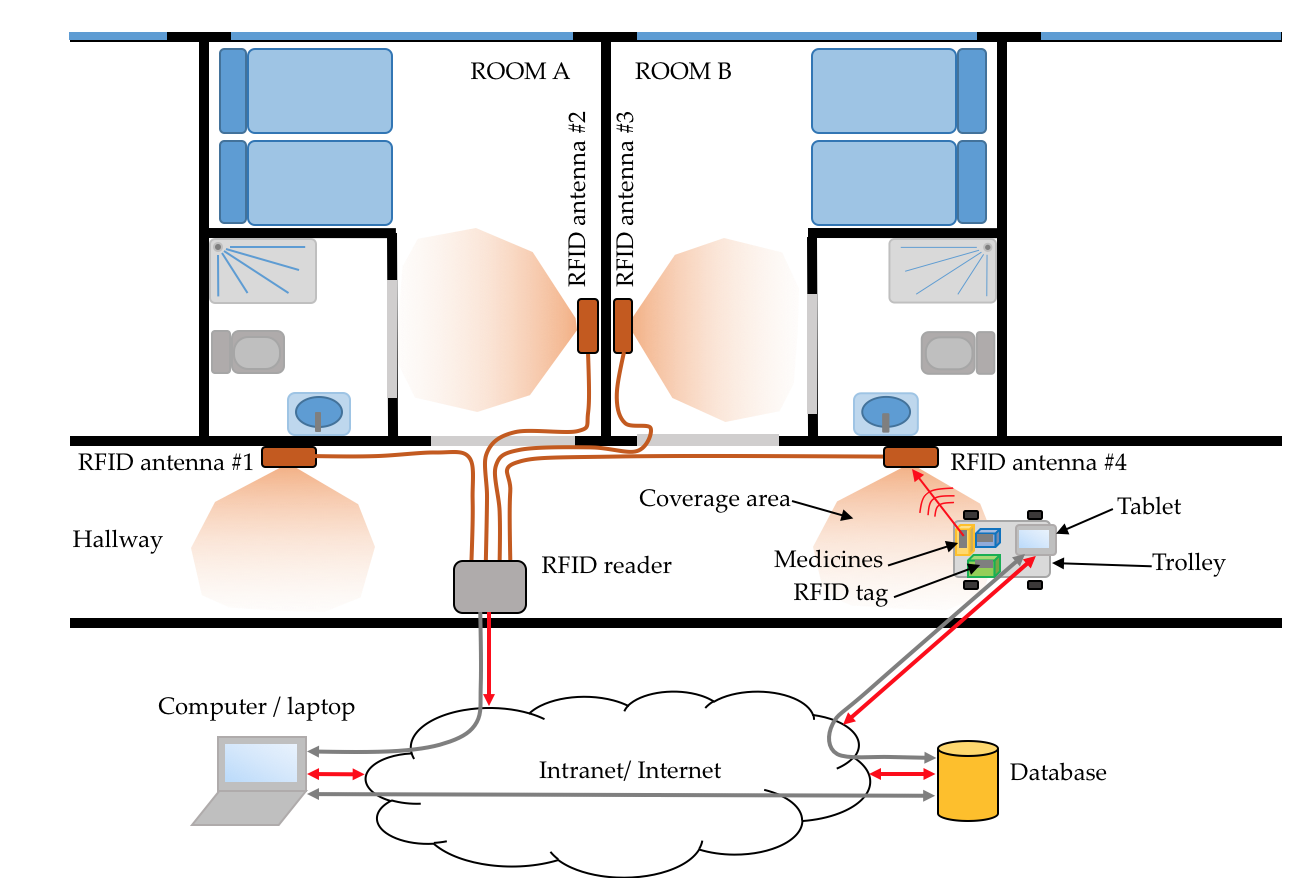
\includegraphics[width=\textwidth]{app_scenario} 
\caption{\label{fig:appfunctionality}User scenario of RFID application} 
\end{figure}

Figure \ref{fig:app_screenshot} shows three screenshots of the developed application. The left picture shows the initial window containing a list of all drugs which were detected by the RFID reader and are stored in the database. The screenshot in the middle shows the screen after selecting one drug of the start page. It gives further information of the selected item. Each drug is stored with an 'ID' (which is the same as the RFID tag number). The 'Countrycode' attribute refers to the country-specific number of each drug. For example, in Germany 'Aspirin' has a specific unique code which is called \ac{PZN}, and contains a 7- or 8-place number (e.g. 04114918). The 'Location' attribute describes the exact location of a drug and refers to the location system in the stock (e.g. in pharmacies). The information 'Timestamp' refers to the last time a drug was detected. The value on the right side of 'Timestamp' is the default value for storing timestamps in MongoDB. If another date format is required, this can be easily defined in the MongoDB schema definition. The last information about the selected drug, named 'Event', represents the information about a drug being detected by one of the antennas or administered to a patient. If the nurse or doctor selects the button 'Administer to patient', the system checks, if the selected drug is permitted to be administered to the patient in the room or not. If it is permitted, the information about the administered drug will be stored in the database and the content of the 'Event' changes to 'Administered to patient in room XX'.

\begin{figure}
\centering
\subfigure[Initial page of application]{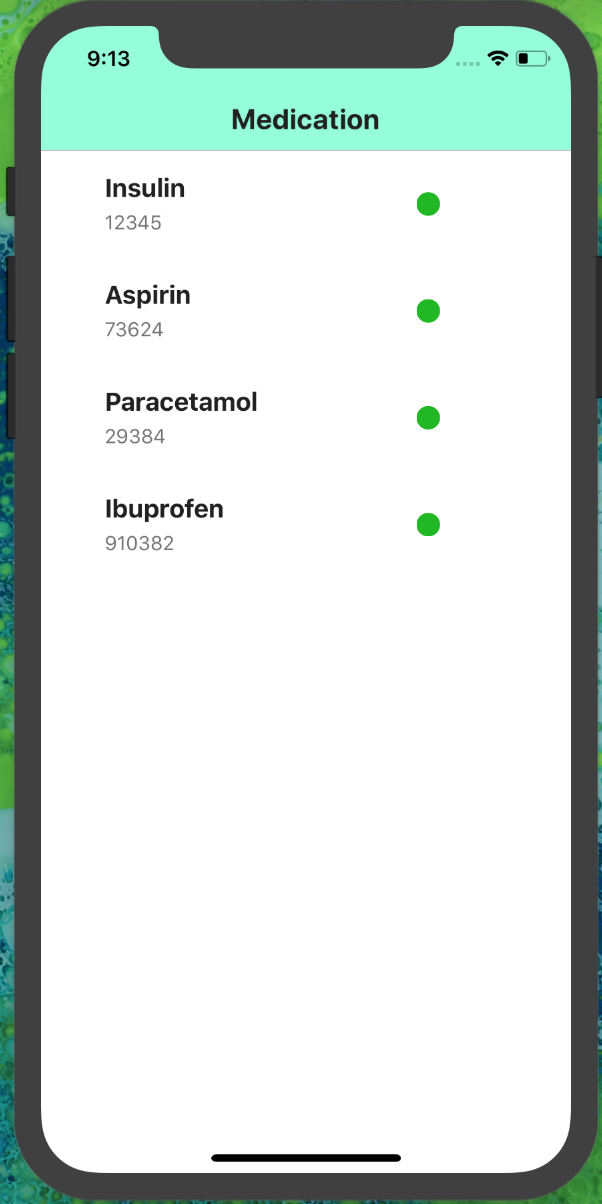
\includegraphics[width=4cm, height=8cm]{Mainview}}
\subfigure[Item information page]{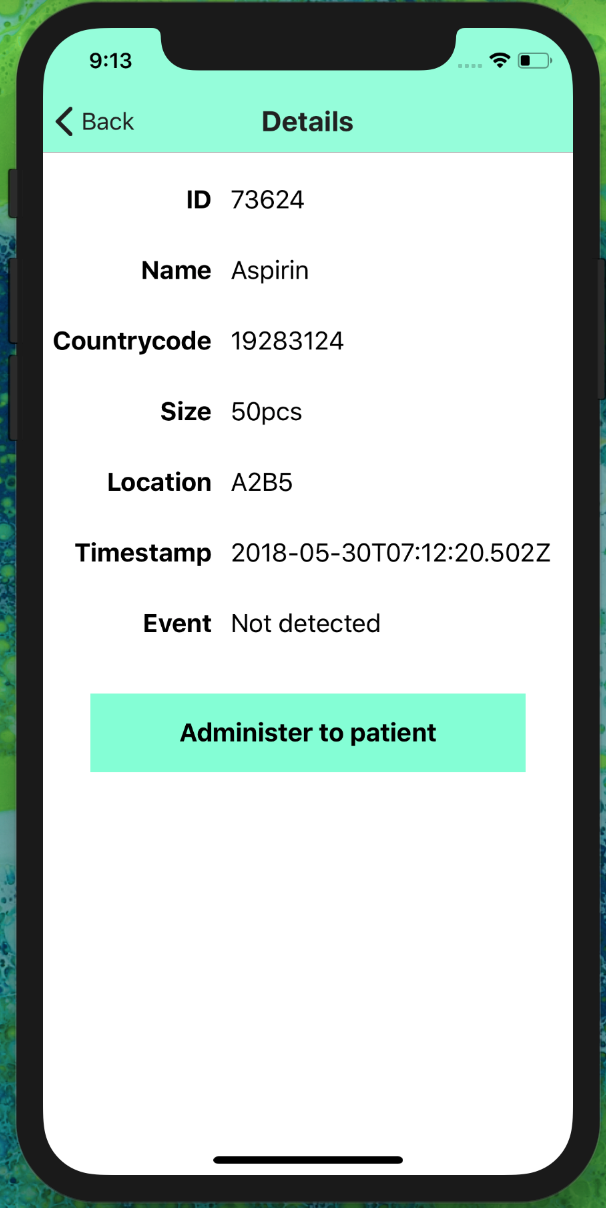
\includegraphics[width=4cm, height=8cm]{Detailview}}
\subfigure[Information about administered drug to patient]{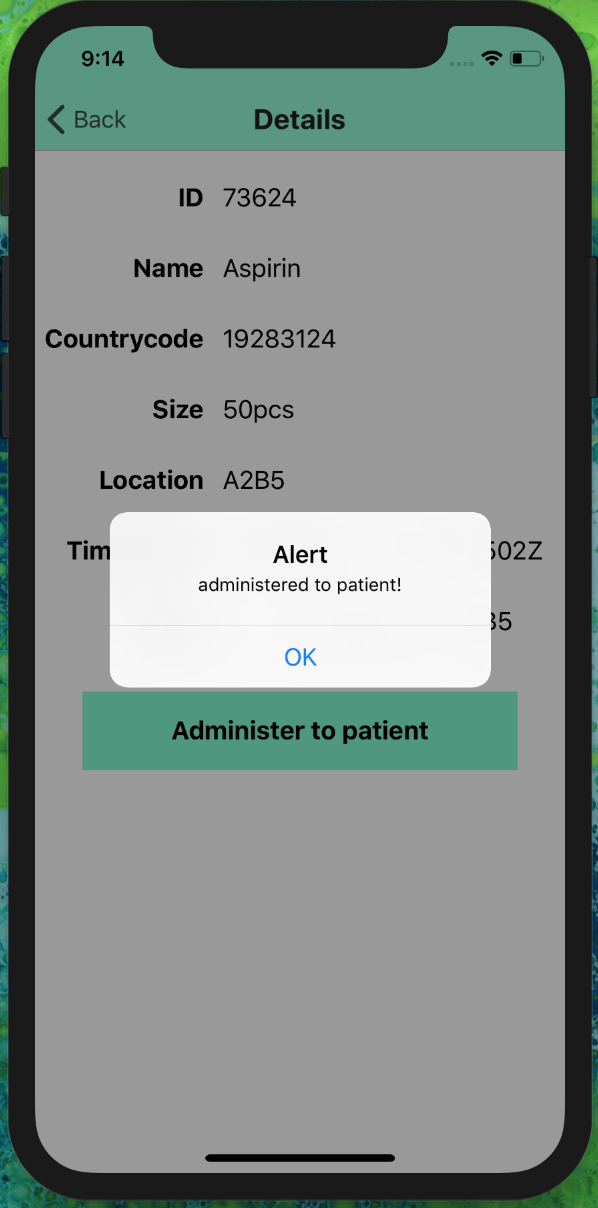
\includegraphics[width=4cm, height=8cm]{administeredView}}
\caption{\label{fig:app_screenshot}Layout of application, Screenshot of iOS Simulator}
\end{figure}

\subsection{Software Architecture} \label{section_architecture}

The following section focuses on the system's architecture which can be seen on figure \ref{fig:apparchitecture}. In the top right corner, the drugs and patients which can be tagged with a RFID tag are displayed. When approaching an antenna, information about medication (e.g. stock availability ect.) is transmitted. At the same time, the RFID reader registers the detected tag and captures its information using Matlab. Matlab synchronizes the transmitted information with the MongoDB database. When receiving current drug information, the server instance sends the data through a Socket.IO connection to the client (smartphone or tablet). Synchronously, all data is transmitted and displayed on the mobile device.

\begin{figure}
\centering
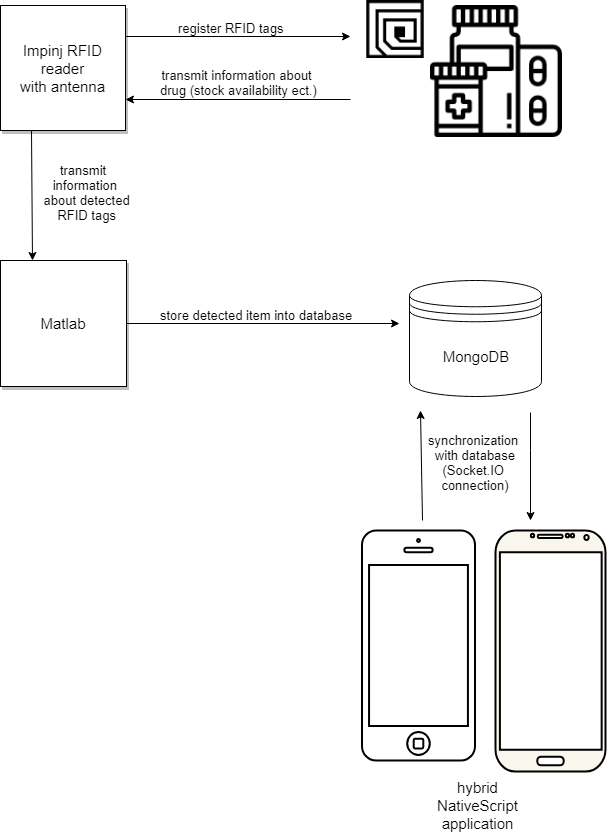
\includegraphics[width=\textwidth]{app_architecture} 
\caption{\label{fig:apparchitecture}The developed system architecture of the mobile RFID application} 
\end{figure}

\subsubsection{Datamodel}

Figure \ref{fig:datamodel} reflects the outline of the developed MongoDB document related to its context and the MongoDB database. As depicted in Figure 4.6, each drug entry contains information about its ID, name, countrycode, size, location, timestamp and event. All documents are pooled in a drug collection which forms a part of medication database. This data model can be extended for example by other collections containing information about several equipment or patients. 

\begin{figure}
\centering
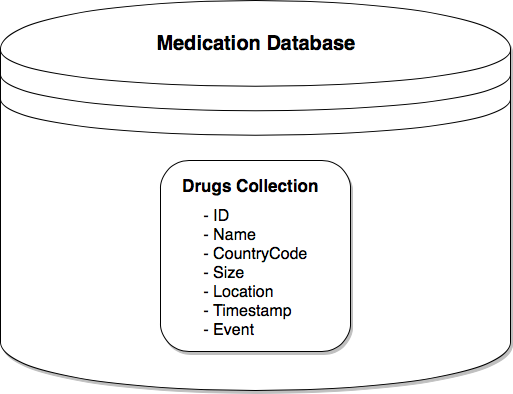
\includegraphics[width=8cm, height=6cm]{Mongo_DataModel} 
\caption{\label{fig:datamodel}Applied data model} 
\end{figure}

\subsubsection{\ac{LAN} Architecture}

Figure \ref{fig:hub_architecture} shows the scheme of the connections between all relevant components into one LAN. There are two networks: On the one hand, the LAN between RFID reader, laptop and desktop PC. On the other hand, a local network between the laptop and various mobile devices, like smartphones or tablets is established. The only connecting point between both networks is the laptop with the IP 169.254.1.2.

At the top of figure \ref{fig:hub_architecture}, there is a '5-Port-Ethernet-Hub' which enables connecting up to five different devices or computers via ethernet. 
On the left of the picture, the RFID reader, with IP 169.254.1.1, is depicted. Each time, when detecting a RFID tag, the RFID reader sends the information to Matlab which is running on the desktop PC with the IP 169.254.1.3. 

After receiving the detected RFID tag's information, the desktop PC transmits the data to MongoDB database running on the laptop with the IP 169.254.1.2. 
The purpose of the second local network between laptop and mobile devices is to execute the NativeScript app and to visualize currently detected RFID tags in the app.

\begin{figure}
\centering
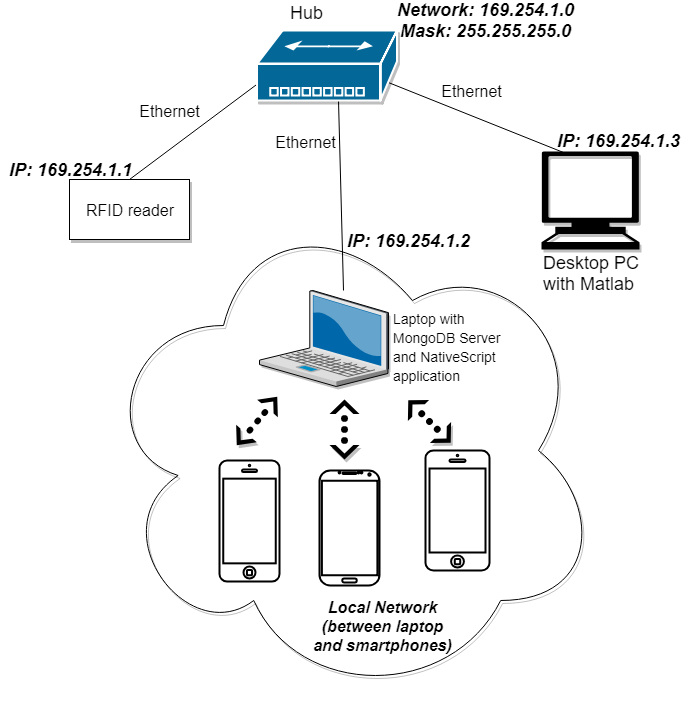
\includegraphics[width=\textwidth]{hub_architecture} 
\caption{\label{fig:hub_architecture}The LAN architecture of the developed system} 
\end{figure}

\subsubsection{Reading Process in Matlab}

The following section focuses on the reading process which is implemented in Matlab. Matlab uses the Impinj Octane SDK \cite{octanesdk} which easily connects the RFID reader to Matlab. The usual reading process in Matlab can be seen in figure \ref{fig:reading_matlab}. In the top left corner of figure \ref{fig:reading_matlab}, after starting the Matlab code, a setup method triggers the initialize method. 

After initializing, Matlab starts reading tags during a predefined time (t). Every time a RFID tag is read, the method eventhandlerChanged() is executed. EventhandlerChanged() notices the changes in the detected tags and triggers a new action 'store data'. After that, analogous to the first concept of the system (see section \ref{firstconcept}), the *.mat data is converted into *.csv data and as such exported. In the most current version of the system, the two last actions (conversion and export) are brought together and data is directly transfered into the MongoDB database. 

\begin{figure}
\centering
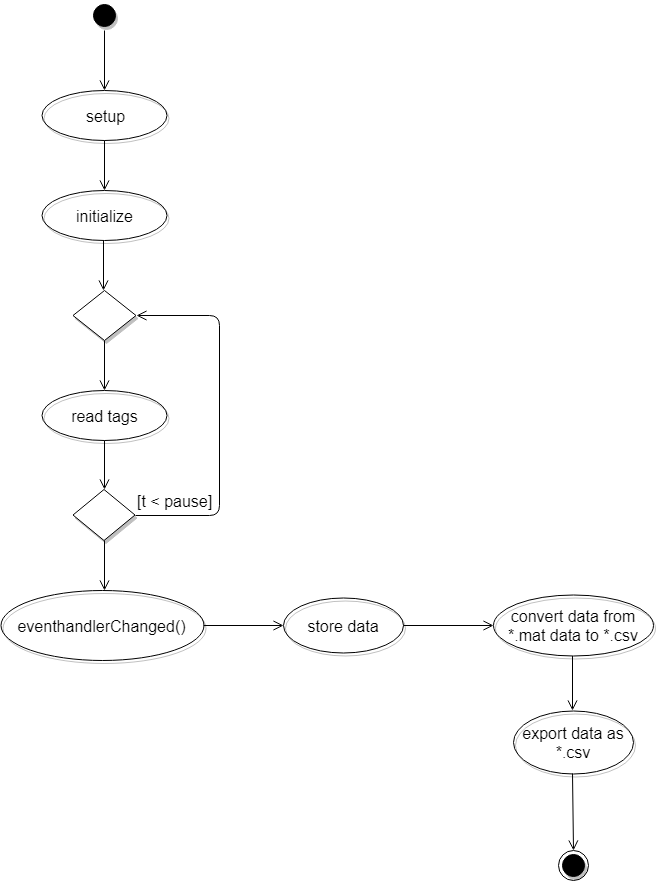
\includegraphics[width=\textwidth]{reading_matlab} 
\caption{\label{fig:reading_matlab}Activity diagram: reading process in Matlab} 
\end{figure}

\section{Tests of system}\label{tests}

\ac{HUCA} located in Oviedo, depends on the 'Servicio de Salud del Principado de Asturias' \cite{huca}. Since 28 February 1990, HUCA has been accredited as University Hospital University Hospital due to the cooperation with the university of Oviedo.

HUCA provides 944 beds, 25 operating suites, 238 rooms for external surgical as well as two gamma cameras (\ac{SPECT}/\ac{TC}) \cite{huca}. Altogether, HUCA is divided into 43 medical services, such as alergology, clinical analysis, clinical biochemistry, general surgery, Nephrology, Neurology, Rehabilitation, prevention of work-related risks, radiodiagnostics etc. 

Besides, HUCA forms a part of the 'unit of national reference for work-related illnesses of the respiratory system'. Together with the 'Hospital Monte Naranco', 'hospital del Área Sanitaria IV' and with reference to \ac{SESPA} 'Servicio de Salud del Principado de Asturias' and finally the 'Instituto Nacional de Silicosis', HUCA promotes research on the subject of respiratory disease and its preventions measures.

Figure \ref{fig:permission} shows the permission letter, signed by the director Gloria Herías Corral of HUCA on 8 May 2018 in Oviedo.
Tests were conducted in June 2018.

\begin{figure}
\centering
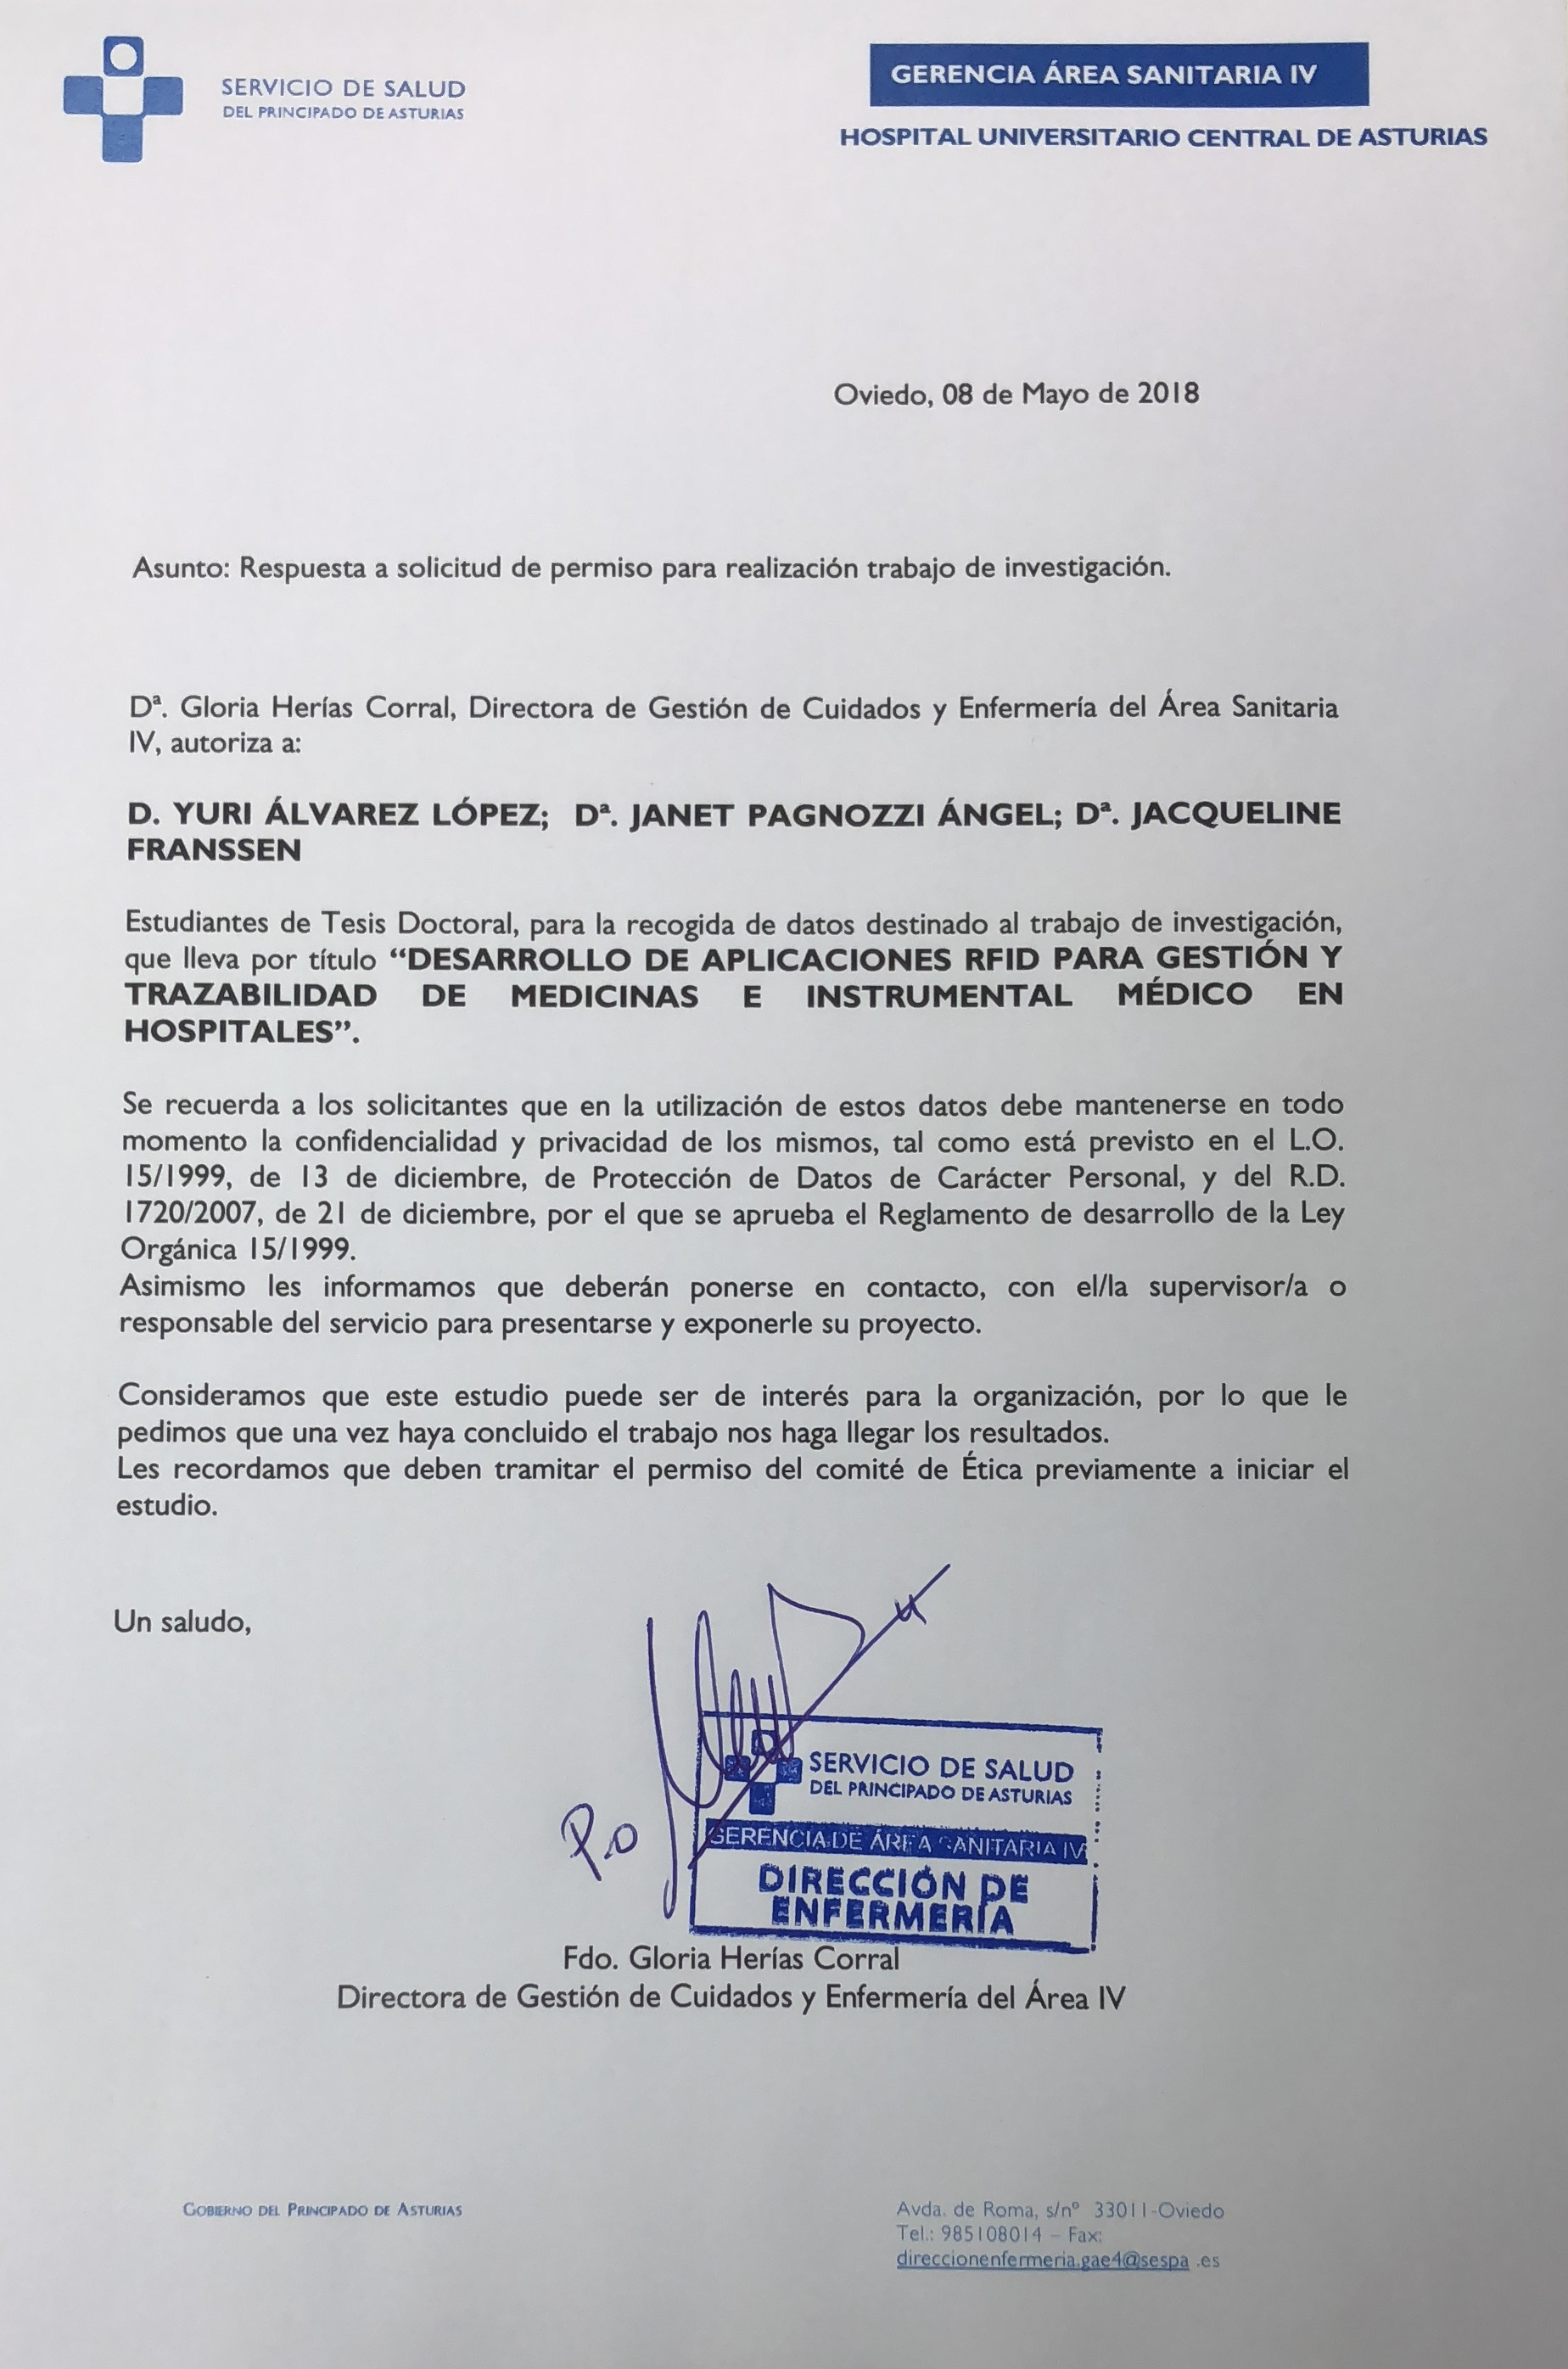
\includegraphics[width=\textwidth]{permission_HUCA} 
\caption{\label{fig:permission}Permission letter about application tests in HUCA} 
\end{figure}

\subsection{Planned tests of system}

\subsubsection{Test scenario}

The following section describes a test scenario. 
The system is devoted to be used in a context where a nurse has to administer several drugs to many patients in a hospital. With the proposed system, the nurse can control and capture each time she is administering a drug to a patient. The system will check if the selected drug (which was detected in the patient's room) is valid and if it can be administered to the patient. For example, the nurse is walking with a trolley (containing several drugs) on the hallway of a department in the hospital. On the hallway, there are two antennas which are connected to a reader installed nearby. When passing close to antennas, the detected drugs will be automatically stored into the MongoDB database and displayed on the mobile phone or tablet. 
When entering the patient's room, a second antenna detects the drugs and transmits the signal to the reader which receives the information about the location of the drug ('drug X detected in room 314'). After that, if the nurse wants to administer a drug, the system checks whether it was already administered and whether it is permissible. After having administered the selected drug, the event will change to 'already administered in room X' and will be stored in the database. 

\subsubsection{Functional tests}

In order to test the real-time synchonization, all entries in the database were deleted and the application was refreshed (by using the pull-to-refresh plugin). After five seconds, the alert dialog which explains that there are no entries in the database and no detected drugs is displayed (tested 06 June 2018). 

\subsubsection{Device test}

The application was tested on four devices including both tablets and smartphones. During development, mainly the iOS simulator was used to rapidly execute and synchronize the application. Since installing a prototype app on an iOS device requires several developer certificates and some configuration steps, it was easier to use the included simulator which is offered by XCode. 
Later, when the app could be executed without throwing any errors, it was installed and tested on an iPhone 7 (Model: 15F79, iOS 11.4). Furthermore, it was installed on an iPad (iOS 11.4) and ran successfully. 
Moreover, the app was tested on two Android devices: a smartphone (Samsung Galaxy S3, Model: GT-9300, Android 4.3) as well as a tablet (Model: Samsung GT-P5110, Android 4.2.2, screen size: 10.1'').
The successful test results can be seen in figure \ref{fig:s3_screenshots}. The figure shows the screenshots of the smartphone "Samsung S3 GT I9300".

\begin{figure}
\centering
\subfigure{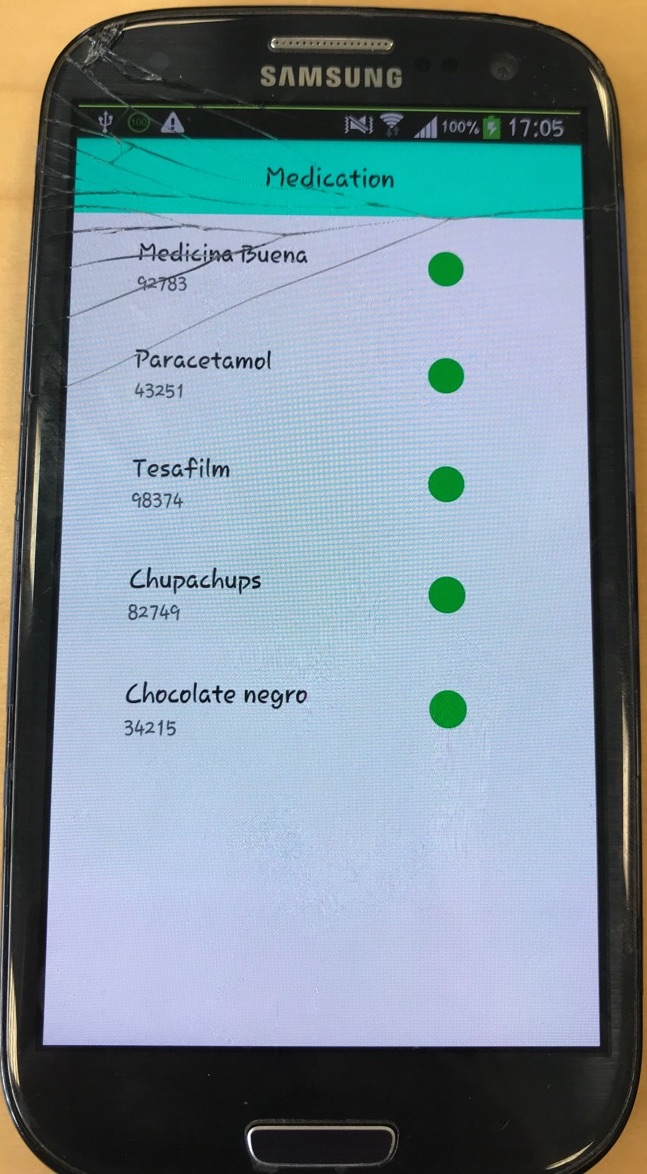
\includegraphics[width=6cm, height=10cm]{s3_01}}
\subfigure{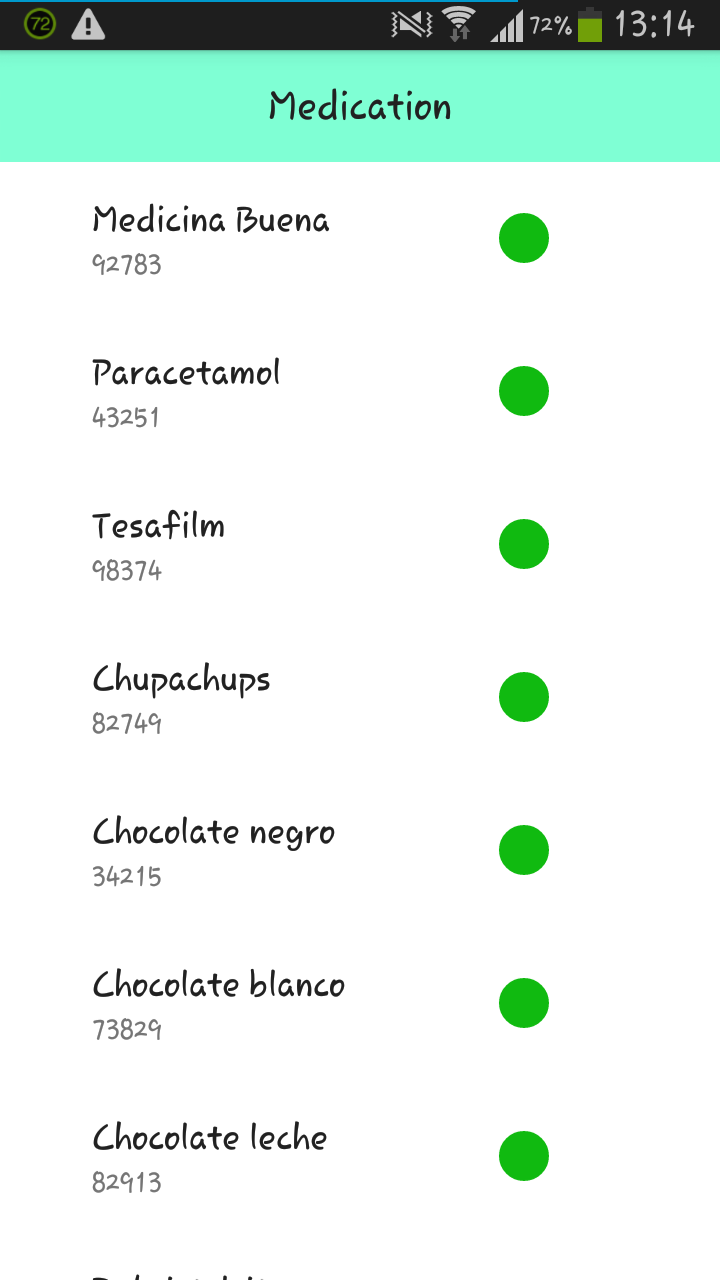
\includegraphics[width=6cm, height=10cm]{s3_02}}
\subfigure{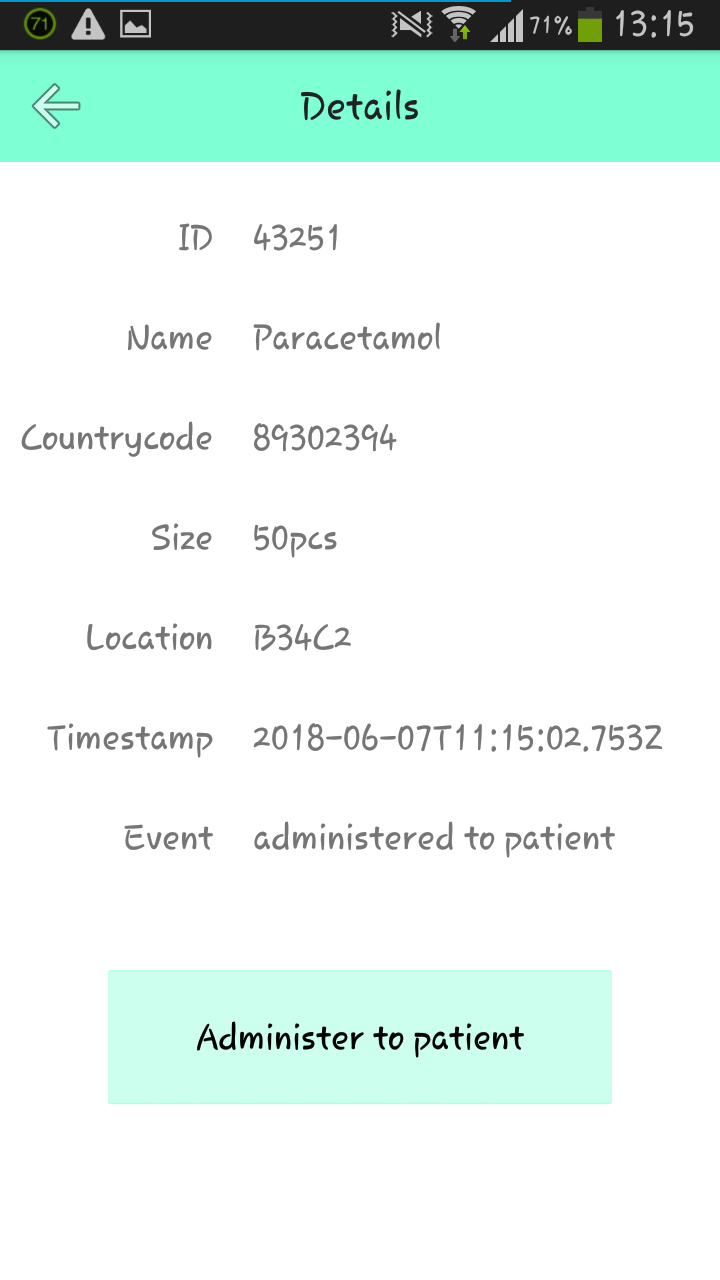
\includegraphics[width=6cm, height=10cm]{s3_03}}
\subfigure{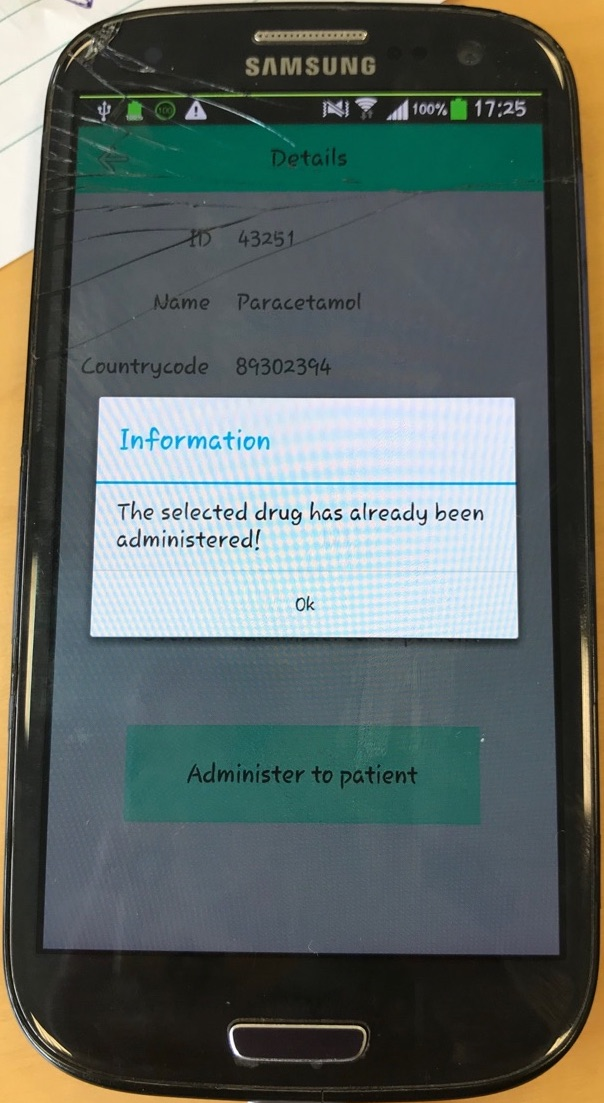
\includegraphics[width=6cm, height=10cm]{s3_04}}
\caption{\label{fig:s3_screenshots} Test screenshots, Samsung S3 GT I9300}
\end{figure}

\subsection{Test results}

\subsection{Evaluation of test results}

During the first tests in the HUCA on Monday, on 25/06/2018, some small features of the application were noticed negatively. For instance, the "real-time" synchronization between the mobile device and the database. The reading process of the RFID reader and the following insertion process into the database did work without problems, but the Socket.IO connection between the mobile client and the database server has to be optimized. Moreover, the feature of pulling down the app to refresh all data turned out to be rather obstructive than useful. To solve this problem, a function which automatically reloads the app's main page has to be implemented. These two features have been successfully fixed in the latest version of the application.

\section{Conclusions and further work}

\subsection{Conclusions}

As mentioned at the beginning of this chapter \ref{requirements}, the aim of this Bachelor Thesis is to improve logistics and the management of drugs in hospitals. By implementing a hybrid mobile application and connecting it to a MongoDB database, a very scalable as well as easy to use solution is purposed.
By implementing a real-time Socket.IO connection between clients and the database server medical staff can check the location and availability of drugs.
The given system offers a secure, approved solution to control the correct administration of drugs to each patient by checking the permission on the server-side. If a drug has been administrated successfully to a patient, it is not possible to repeat the administration. 
Moreover, using a 868 MHz frequency band drugs located on the same floor can be detected. To use the system, drugs need to be tagged with a RFID tag. 
In addition to that, the proposed solution replaces the paper-based administration of drugs to patients and prevents a duplicate administration of drugs or other errors.
Furthermore, the developed system has been established independently from any existing hospital information systems. Therefore, there is no preparation needed for the deployment in any department of hospitals.
To conclude, the given system can also be deployed in other contexts, like for example in schools or universities in order to check the attendance of students in exams (e.g. each student has a unique student's card which is tagged with a RFID tag).

\subsection{Further work}

The developed application can be extended in many ways, that will be described next.

During testing in the HUCA, a nurse mentioned that when administering drugs to patients, she usually has to carry a medicine trolley with several containers, each for a specific patient. Actually, most of the patients in a hospital have to take more than only one drug which has to be organized in a list. In the past, the nurses had to manually check the patient related medication on a paper.
So, in future it would be very useful to divide the application into different sections which are related to a specific patient. This also implies, to change the format of the stored data. To be precisely, each patient could be stored in the MongoDB database as a top level document and contains various subdocuments which are his drugs. Since the structure of these drug documents already exists in the developed application, it would be very easy to adopt and implement that solution. Another possibility would be to connect the application to each electronic patient record, which can be seen in figure \ref{fig:newdatamodel}. Consequently, each patient can be easily identified with its medication list.

\begin{figure}
\centering
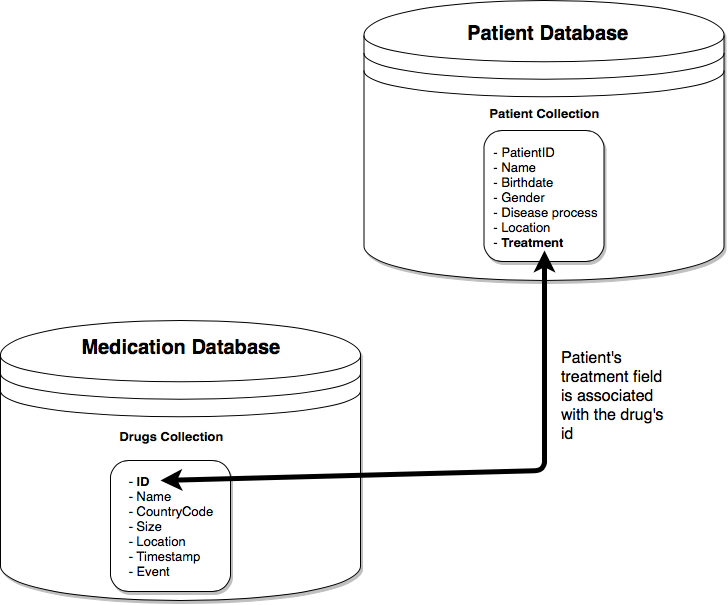
\includegraphics[width=\textwidth]{extension_mongodatamodel} 
\caption{\label{fig:newdatamodel}Example of extended data model, each patient entry is associated to the medication list} 
\end{figure}

Furthermore, in case of a patient's room where two or more patients are accomodated, the system should distinguish between those. To fastly identify a patient and its related medication on the medicine trolley, one solution could be to let patients wear a wristband with the same passive RFID tag as the drugs. Each time, the same antenna detects a drug and the patients wristband, it checks whether the drug should be administered to the patient and either allows the administration or not.

Another possible scenario would be to set up user roles in the application. This means, that for example the chief physician or the head of nurses sets up a list of medication related to each patient and only this person has access to the personal data. To provide patient's safety, there should be no other nurse or stuff in the hospital who can access the patient's related medication data. After setting up the drugs and its permissions to be administered to the specific patients, this "administrator" saves all data and logs out. 
Apart from this administrator, there will be another account, such as "nurse" or any ordinary user account. This person administers the drugs to each patients.